% Options for packages loaded elsewhere
\PassOptionsToPackage{unicode}{hyperref}
\PassOptionsToPackage{hyphens}{url}
\PassOptionsToPackage{dvipsnames,svgnames,x11names}{xcolor}
%
\documentclass[
  letterpaper,
  DIV=11,
  numbers=noendperiod]{scrreprt}

\usepackage{amsmath,amssymb}
\usepackage{lmodern}
\usepackage{iftex}
\ifPDFTeX
  \usepackage[T1]{fontenc}
  \usepackage[utf8]{inputenc}
  \usepackage{textcomp} % provide euro and other symbols
\else % if luatex or xetex
  \usepackage{unicode-math}
  \defaultfontfeatures{Scale=MatchLowercase}
  \defaultfontfeatures[\rmfamily]{Ligatures=TeX,Scale=1}
\fi
% Use upquote if available, for straight quotes in verbatim environments
\IfFileExists{upquote.sty}{\usepackage{upquote}}{}
\IfFileExists{microtype.sty}{% use microtype if available
  \usepackage[]{microtype}
  \UseMicrotypeSet[protrusion]{basicmath} % disable protrusion for tt fonts
}{}
\makeatletter
\@ifundefined{KOMAClassName}{% if non-KOMA class
  \IfFileExists{parskip.sty}{%
    \usepackage{parskip}
  }{% else
    \setlength{\parindent}{0pt}
    \setlength{\parskip}{6pt plus 2pt minus 1pt}}
}{% if KOMA class
  \KOMAoptions{parskip=half}}
\makeatother
\usepackage{xcolor}
\setlength{\emergencystretch}{3em} % prevent overfull lines
\setcounter{secnumdepth}{5}
% Make \paragraph and \subparagraph free-standing
\ifx\paragraph\undefined\else
  \let\oldparagraph\paragraph
  \renewcommand{\paragraph}[1]{\oldparagraph{#1}\mbox{}}
\fi
\ifx\subparagraph\undefined\else
  \let\oldsubparagraph\subparagraph
  \renewcommand{\subparagraph}[1]{\oldsubparagraph{#1}\mbox{}}
\fi


\providecommand{\tightlist}{%
  \setlength{\itemsep}{0pt}\setlength{\parskip}{0pt}}\usepackage{longtable,booktabs,array}
\usepackage{calc} % for calculating minipage widths
% Correct order of tables after \paragraph or \subparagraph
\usepackage{etoolbox}
\makeatletter
\patchcmd\longtable{\par}{\if@noskipsec\mbox{}\fi\par}{}{}
\makeatother
% Allow footnotes in longtable head/foot
\IfFileExists{footnotehyper.sty}{\usepackage{footnotehyper}}{\usepackage{footnote}}
\makesavenoteenv{longtable}
\usepackage{graphicx}
\makeatletter
\def\maxwidth{\ifdim\Gin@nat@width>\linewidth\linewidth\else\Gin@nat@width\fi}
\def\maxheight{\ifdim\Gin@nat@height>\textheight\textheight\else\Gin@nat@height\fi}
\makeatother
% Scale images if necessary, so that they will not overflow the page
% margins by default, and it is still possible to overwrite the defaults
% using explicit options in \includegraphics[width, height, ...]{}
\setkeys{Gin}{width=\maxwidth,height=\maxheight,keepaspectratio}
% Set default figure placement to htbp
\makeatletter
\def\fps@figure{htbp}
\makeatother
\newlength{\cslhangindent}
\setlength{\cslhangindent}{1.5em}
\newlength{\csllabelwidth}
\setlength{\csllabelwidth}{3em}
\newlength{\cslentryspacingunit} % times entry-spacing
\setlength{\cslentryspacingunit}{\parskip}
\newenvironment{CSLReferences}[2] % #1 hanging-ident, #2 entry spacing
 {% don't indent paragraphs
  \setlength{\parindent}{0pt}
  % turn on hanging indent if param 1 is 1
  \ifodd #1
  \let\oldpar\par
  \def\par{\hangindent=\cslhangindent\oldpar}
  \fi
  % set entry spacing
  \setlength{\parskip}{#2\cslentryspacingunit}
 }%
 {}
\usepackage{calc}
\newcommand{\CSLBlock}[1]{#1\hfill\break}
\newcommand{\CSLLeftMargin}[1]{\parbox[t]{\csllabelwidth}{#1}}
\newcommand{\CSLRightInline}[1]{\parbox[t]{\linewidth - \csllabelwidth}{#1}\break}
\newcommand{\CSLIndent}[1]{\hspace{\cslhangindent}#1}

\KOMAoption{captions}{tableheading}
\makeatletter
\makeatother
\makeatletter
\@ifpackageloaded{bookmark}{}{\usepackage{bookmark}}
\makeatother
\makeatletter
\@ifpackageloaded{caption}{}{\usepackage{caption}}
\AtBeginDocument{%
\ifdefined\contentsname
  \renewcommand*\contentsname{Table of contents}
\else
  \newcommand\contentsname{Table of contents}
\fi
\ifdefined\listfigurename
  \renewcommand*\listfigurename{List of Figures}
\else
  \newcommand\listfigurename{List of Figures}
\fi
\ifdefined\listtablename
  \renewcommand*\listtablename{List of Tables}
\else
  \newcommand\listtablename{List of Tables}
\fi
\ifdefined\figurename
  \renewcommand*\figurename{Figure}
\else
  \newcommand\figurename{Figure}
\fi
\ifdefined\tablename
  \renewcommand*\tablename{Table}
\else
  \newcommand\tablename{Table}
\fi
}
\@ifpackageloaded{float}{}{\usepackage{float}}
\floatstyle{ruled}
\@ifundefined{c@chapter}{\newfloat{codelisting}{h}{lop}}{\newfloat{codelisting}{h}{lop}[chapter]}
\floatname{codelisting}{Listing}
\newcommand*\listoflistings{\listof{codelisting}{List of Listings}}
\makeatother
\makeatletter
\@ifpackageloaded{caption}{}{\usepackage{caption}}
\@ifpackageloaded{subcaption}{}{\usepackage{subcaption}}
\makeatother
\makeatletter
\@ifpackageloaded{tcolorbox}{}{\usepackage[many]{tcolorbox}}
\makeatother
\makeatletter
\@ifundefined{shadecolor}{\definecolor{shadecolor}{rgb}{.97, .97, .97}}
\makeatother
\makeatletter
\makeatother
\ifLuaTeX
  \usepackage{selnolig}  % disable illegal ligatures
\fi
\IfFileExists{bookmark.sty}{\usepackage{bookmark}}{\usepackage{hyperref}}
\IfFileExists{xurl.sty}{\usepackage{xurl}}{} % add URL line breaks if available
\urlstyle{same} % disable monospaced font for URLs
\hypersetup{
  pdftitle={Toward automatic preprocessing of complex free response data},
  pdfauthor={Jordan Gunn},
  colorlinks=true,
  linkcolor={blue},
  filecolor={Maroon},
  citecolor={Blue},
  urlcolor={Blue},
  pdfcreator={LaTeX via pandoc}}

\title{Toward automatic preprocessing of complex free response data}
\author{Jordan Gunn}
\date{}

\begin{document}
\maketitle
\begin{abstract}
This paper explores the potential of automatic natural language
processing (NLP) techniques for preprocessing complex free response data
in domains pertinent to psychological research. We break down the task
of coding free response data into discrete preprocessing steps such as
text segmentation, response unit matching, and sequence identification
and examine a range of applicable technologies for performing them. Our
findings reveal that compared to a baseline approach where sentences in
a response are independently compared to target items for matching, a
more effective sequence can be established when contextualized
embeddings are used for comparing response units to target items.
Furthermore, considering every possible subsequence of the response,
rather than segmenting responses by sentence, significantly improves
candidate matchings. We conclude with a discussion of the challenges and
opportunities for automated free response data analysis and propose
future research avenues to further refine these techniques.
\end{abstract}
\ifdefined\Shaded\renewenvironment{Shaded}{\begin{tcolorbox}[interior hidden, enhanced, borderline west={3pt}{0pt}{shadecolor}, boxrule=0pt, breakable, sharp corners, frame hidden]}{\end{tcolorbox}}\fi

\renewcommand*\contentsname{Table of contents}
{
\hypersetup{linkcolor=}
\setcounter{tocdepth}{2}
\tableofcontents
}
\bookmarksetup{startatroot}

\hypertarget{section}{%
\chapter{}\label{section}}

Free response data consist of unstructured, open-ended answers generated
by individuals responding to prompts or cues. Unlike structured data,
collected through closed-ended probes that provide limited response
options, research participants produce free response data in their own
words, enabling additional insight into their thought processes and
mental representations. In research across various fields such as
psychology, sociology, and education, free response data is often
analyzed qualitatively to understand participants' complex and varied
experiences, attitudes, and perspectives (Hollway \& Jefferson, 2000).
In cognitive science, qualitative research methods are comparatively
rare, but free response data is nonetheless central to the study of the
mental processes underlying human behavior. Quantitative analyses of the
ordering of freely generated responses and the time taken to produce
them have provided key constraints for accounts of how people retrieve
information from memory, make decisions, and solve problems (Ericsson,
2006; Kahana, 2020).

Free response data has been particularly influential in the study of
memory search. For example, in the free recall task, participants are
asked to remember a list of studied items in the order they come to
mind. Data from the free recall paradigm reliably exhibits a temporal
contiguity effect, in which items studied near one another are more
likely to be associated and retrieved near one another. Experiments and
analyses confirming this effect's time-scale invariance, automaticity,
and forward-asymmetry are central to ongoing debates about the
mechanisms underlying search through episodic memory (Healey et al.,
2019). Similarly, in the semantic fluency task, participants are
prompted to generate as many exemplars as possible that belong to a
specified category. The order of responses in the semantic fluency task
has fueled debate about whether semantic memory is typically searched
through a random walk, optimal foraging, or another process (Kumar,
2021).

For free response data in these and many other domains, initial steps
for preprocessing free response data to support organizational analysis
can be broken down into solving two problems: (1) segmenting the
response into discrete units of text (``response units'') and (2)
matching these units to the set of target items or features being
researched. In the free recall task, for example, the text of a
participant's free recall response is segmented into units corresponding
to the words or phrases that participants generate in response to the
prompt. In the semantic fluency task, the text of a participant's
response is segmented into units of text corresponding to the words or
phrases that participants generate in response to the prompt. In both
cases, the units of text are then matched to elements in a set of target
items; these are defined as the items studied in the encoding phase in
the free recall task and as the pool of exemplars or features relevant
to a cue in the semantic fluency task. Response units that cannot be
matched to target items are discarded or considered intrusions. The
result for each set of responses is a sequence of target items
considered to be generated by participants in the order they appear in
the sequence.

While coding data in this way is straightforward enough for
preprocessing small datasets, these demands forestall the use of free
response paradigms in large-scale studies involving large quantities of
participants and designs involving many trials per participant.
Additionally, manual segmentation and correspondence can introduce bias
and inconsistencies into the data, leading to inaccurate results.
Preprocessing is all the more challenging in free response tasks
involving the production of narratives, concepts, or autobiographical
accounts where structured multi-word responses constitute the unit of
scientific interest. Complex free response data such as this require
sensitivity to grammatical conventions and semantic content to
appropriately segment into ordered response units and correspond with
target items. Standards for coding such data are necessarily vague,
often requiring multiple reviewers to preprocess the same data samples
to confirm interrater reliability. Even when these measures are taken,
subtle differences in rater interpretation of these standards contribute
to research degrees of freedom that can make it harder to interpret
results and compare findings across studies (Simmons et al., 2016). An
increasing emphasis on organizational analyses in memory research and
other domains makes it especially urgent to address these limitations
and develop methods for more efficient preprocessing of free response
data.

Over much of the work using free response data, these problems have
mainly been insurmountable, with researchers either relying on manual
coding of free response data or, especially for larger-scale datasets,
focusing on more structured paradigms. However, a cascade of
technological advances in automatic natural language processing (NLP)
has raised the possibility that many aspects of the work involved in
preprocessing complex free response data can be automated, with human
raters perhaps focused on confirming or correcting outputs.

When these technologies work well, NLP has several advantages over
manual methods for preprocessing free response data.

Techniques leveraging this technology have already been proposed for
preprocessing less complex outputs, such as a free recall of word lists
(for example, see). However, manual coding remains the standard approach
to preprocessing complex free response data as ordered sequences of
generated target units suitable for organizational analysis.

A range of NLP techniques has been developed that may be suitable for
the two core problems of preprocessing complex free response data for
organizational analysis. When it comes to segmenting complex discourse
structures (rather than sequences of semantically independent words),

In this paper, we examine the suitability of NLP for preprocessing
complexly structured free response data and provide a brief overview of
state of the art in automated free response data analysis. We develop a
framework that decomposes the task of coding complex free response data
into a sequence of discrete preprocessing steps and identifies
techniques that may automate these activities. Focusing on a few
especially promising approaches, we evaluate these techniques for data
pre-processing across a range of free-response datasets, including free
recall and word sense semantic fluency. We separately compare human and
computational methods for segmenting free response data into units of
text, corresponding response units with target items, and identifying
the ordered sequence of target items generated in a trial. We conclude
by discussing challenges and opportunities for automated free response
data analysis and identifying areas for future research.

\bookmarksetup{startatroot}

\hypertarget{loading-data}{%
\chapter{Loading Data}\label{loading-data}}

Formatting data for use with a new library can be a time consuming
process. If you're using multiple libraries with different data
requirements, you may find yourself reformatting the same data multiple
times, storing multiple copies of the same data in different formats,
and struggling to synchronize changes between them. Rather than
requiring users to reformat their data to fit the library, we we borrow
an approach from \href{https://pytorch.org/}{Pytorch}. Instead of
requiring data be specified in a specific way, Pytorch provides an
abstract Dataset class that can be extended to provide a common
interface for loading data from a variety of sources. Instead of
generating the dataset in a new format, the job becomes to provide
functions retrieve data samples from the original source and return them
in the appropriate format.

Here we outline this approach in more detail (often cribbing from the
Pytorch documentation) and provide examples of how we have used it to
load data in our own research. More specific instructions about what
information a Dataset should return to work with applicable functions
our library will be provided in their specific documentation.

\hypertarget{the-dataset-class}{%
\section{The Dataset Class}\label{the-dataset-class}}

As a toy example, the following class specifies the interface for a
dataset that accesses a text file and treats each line as a separate
sample to be represented as a Markdown object.

We can use it to consider lines of this project's README.

\hypertarget{senses-dataset}{%
\section{Senses Dataset}\label{senses-dataset}}

For trials defining this dataset, participants were cued with a word and
asked to generate all the senses of that word that they could think of.
The dataset is organized as an HDF5 file paired with a text file
containing the pool of senses that participants could generate.

Each item returned by this dataset is a dictionary with the following
keys:

\begin{itemize}
\tightlist
\item
  \texttt{target\_context}: the story text
\item
  \texttt{target\_items}: a list of dictionaries, each representing a
  target item in the story.
\item
  \texttt{response\_transcript}: the response transcript\\
\item
  \texttt{response\_units}: a list of dictionaries, each representing a
  response unit in the response transcript.
\item
  \texttt{matches}: a boolean matrix indicating which response units
  match which target items
\end{itemize}

Each dictionary specified by a target item or response unit has the
following keys:

\begin{itemize}
\tightlist
\item
  \texttt{text}: the text of the target item\\
\item
  \texttt{spans}: a list of tuples, each representing a span of the
  target item in the story text
\end{itemize}

\hypertarget{sbs-narrative-recall-dataset}{%
\section{SBS Narrative Recall
Dataset}\label{sbs-narrative-recall-dataset}}

In this dataset, participants perform free recall of a story they
previously read. The dataset is organized into a directory of text files
and spreadsheets that variously represent encoded stories, participant
responses, and coding decisions made by the lab.

Each item returned by this Dataset is structured similarly to those
returned by the Senses Dataset.

\hypertarget{json-dataset}{%
\section{JSON Dataset}\label{json-dataset}}

To store sequences for downstream evaluation, we'll use the JSON format.

\bookmarksetup{startatroot}

\hypertarget{demo}{%
\chapter{Demo}\label{demo}}

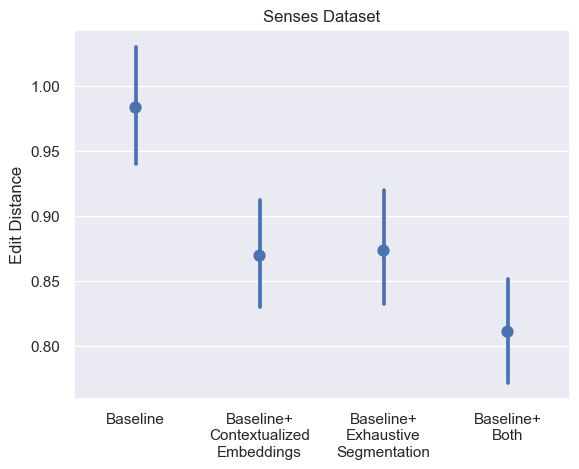
\includegraphics{src/analyses/Comparison_files/figure-pdf/cell-5-output-1.png}

\bookmarksetup{startatroot}

\hypertarget{references}{%
\chapter{References}\label{references}}

\hypertarget{refs}{}
\begin{CSLReferences}{1}{0}
\leavevmode\vadjust pre{\hypertarget{ref-ericsson2006protocol}{}}%
Ericsson, K. A. (2006). Protocol analysis and expert thought: Concurrent
verbalizations of thinking during experts' performance on representative
tasks. \emph{The Cambridge Handbook of Expertise and Expert
Performance}, 223--241.

\leavevmode\vadjust pre{\hypertarget{ref-healey2019contiguity}{}}%
Healey, M. K., Long, N. M., \& Kahana, M. J. (2019). Contiguity in
episodic memory. \emph{Psychonomic Bulletin \& Review}, \emph{26}(3),
699--720.

\leavevmode\vadjust pre{\hypertarget{ref-hollway2000doing}{}}%
Hollway, W., \& Jefferson, T. (2000). \emph{Doing qualitative research
differently: Free association, narrative and the interview method}.
Sage.

\leavevmode\vadjust pre{\hypertarget{ref-kahana2020computational}{}}%
Kahana, M. J. (2020). Computational models of memory search.
\emph{Annual Review of Psychology}, \emph{71}, 107--138.

\leavevmode\vadjust pre{\hypertarget{ref-kumar2021semantic}{}}%
Kumar, A. A. (2021). Semantic memory: A review of methods, models, and
current challenges. \emph{Psychonomic Bulletin \& Review}, \emph{28},
40--80.

\leavevmode\vadjust pre{\hypertarget{ref-simmons2016false}{}}%
Simmons, J. P., Nelson, L. D., \& Simonsohn, U. (2016).
\emph{False-positive psychology: Undisclosed flexibility in data
collection and analysis allows presenting anything as significant.}

\end{CSLReferences}



\end{document}
